\begin{enumerate}

\item Consider the numbers from 1 to 10.  Give the set of pairs of these numbers that 
corresponds to the divisibility relation.

\vfill

\hint{A pair is ``in'' the relation when the first number gazinta the second number.  $1$ gazinta anything, $2$ gazinta the even numbers, $3$ gazinta $3$, $6$ and $9$, etc. (Also a number always gazinta itself.)}

\vfill

\item The \index{domain}\emph{domain} of a function (or binary relation) 
is the set of numbers appearing in the first coordinate.  The \index{range} 
\emph{range} of a function (or binary relation) is the set of numbers 
appearing in the second coordinate.  

Consider the set $\{0,1,2,3,4,5,6\}$ and the function $f(x) = x^2 \pmod{7}$.
Express this function as a relation by explicitly writing out the set of
ordered pairs it contains.  What is the range of this function?
 
 \vfill
 
\hint{
\[ f \; = \; \{(0,0), (1,1), (2,4), (3,2), (4,2), (5,4), (6,1)\} \]
\[ \Rng{f} \;= \; \{0,1,2,4\} \]

}

\vfill

\workbookpagebreak
\hintspagebreak

\item What relation on the numbers from 1 to 10 does the following set of ordered pairs
represent?

\begin{gather*}
\{ (1,1), (1,2), (1,3), (1,4), (1,5), (1,6), (1,7), (1,8), (1,9), (1,10), \\
(2,2), (2,3), (2,4), (2,5), (2,6), (2,7), (2,8), (2,9), (2,10), \\
(3,3), (3,4), (3,5), (3,6), (3,7), (3,8), (3,9), (3,10), \\
(4,4), (4,5), (4,6), (4,7), (4,8), (4,9), (4,10), \\
(5,5), (5,6), (5,7), (5,8), (5,9), (5,10), \\
(6,6), (6,7), (6,8), (6,9), (6,10), \\
(7,7), (7,8), (7,9), (7,10), \\
(8,8), (8,9), (8,10), \\
(9,9), (9,10), \\
(10,10) \} 
\end{gather*}

\vfill

\hint{ Less-than-or-equal-to }

\vfill

\hintspagebreak
\workbookpagebreak

\item Draw a five-pointed star, label all 10 points. There are 40 triples of these 
labels that satisfy the betweenness relation.  List them.

\vfill

\hint{
Yeah, hmmm. Forty is kind of a lot...
Let's look at the points (E,F,G and B) on the horizontal line in the diagram below. The triples involving these four points are: (E,F,G), (G,F,E), (E,F,B), (B,F,E), (E,G,B), (B,G,E), (F,G,B), (B,G,F).

\vfill

\centerline{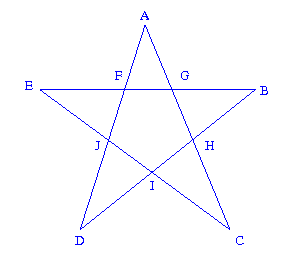
\includegraphics{figures/star}}

\vfill

}

\workbookpagebreak

\item Sketch a graph of the relation 
\[
\{ (x,y) \suchthat x,y \in \Reals \; \mbox{and} \; y > x^2 \}.
\]

\hint{Is this the region above or below the curve $y=x^2$?}

\wbvfill

\item A function $f(x)$ is said to be \index{invertible function} 
\emph{invertible} if there is another function $g(x)$ such that 
$g(f(x)) = x$ for all values of $x$.  (Usually, the inverse function,
$g(x)$ would be denoted $f^{-1}(x)$.)   Suppose a function is presented 
to you as a relation -- that is, you are just given a set of pairs.  
How can you distinguish whether the function represented by this list 
of input/output pairs is invertible?  How can you produce the inverse 
(as a set of ordered pairs)?
 
\hint{If $f$ sends $x$ to $y$, then we want $f^{-1}$ to send $y$ back to $x$.  So the inverse just has the pairs in $f$ reversed.  When is the inverse going to fail to be a function?}

\wbvfill

\workbookpagebreak

\item There is a relation known as ``has color'' which goes from the
set 
\[ F = \{orange, cherry, pumpkin, banana\} \]
to the set 
\[ C = \{orange, red, green, yellow\}. \]

\noindent  What pairs are in ``has color''?
   
\hint{Depending on your personal experience level with fruit there may be different answers.  Certainly
(orange, orange) will be one of the pairs, but (orange, green) happens too!}

\wbvfill

\end{enumerate}
